\documentclass{standalone}
\usepackage{tikz}
\usetikzlibrary{patterns, positioning}
\usepackage[sfdefault]{ClearSans} %% option 'sfdefault' activates Clear Sans as the default text font
\usepackage[T1]{fontenc}

\begin{document}
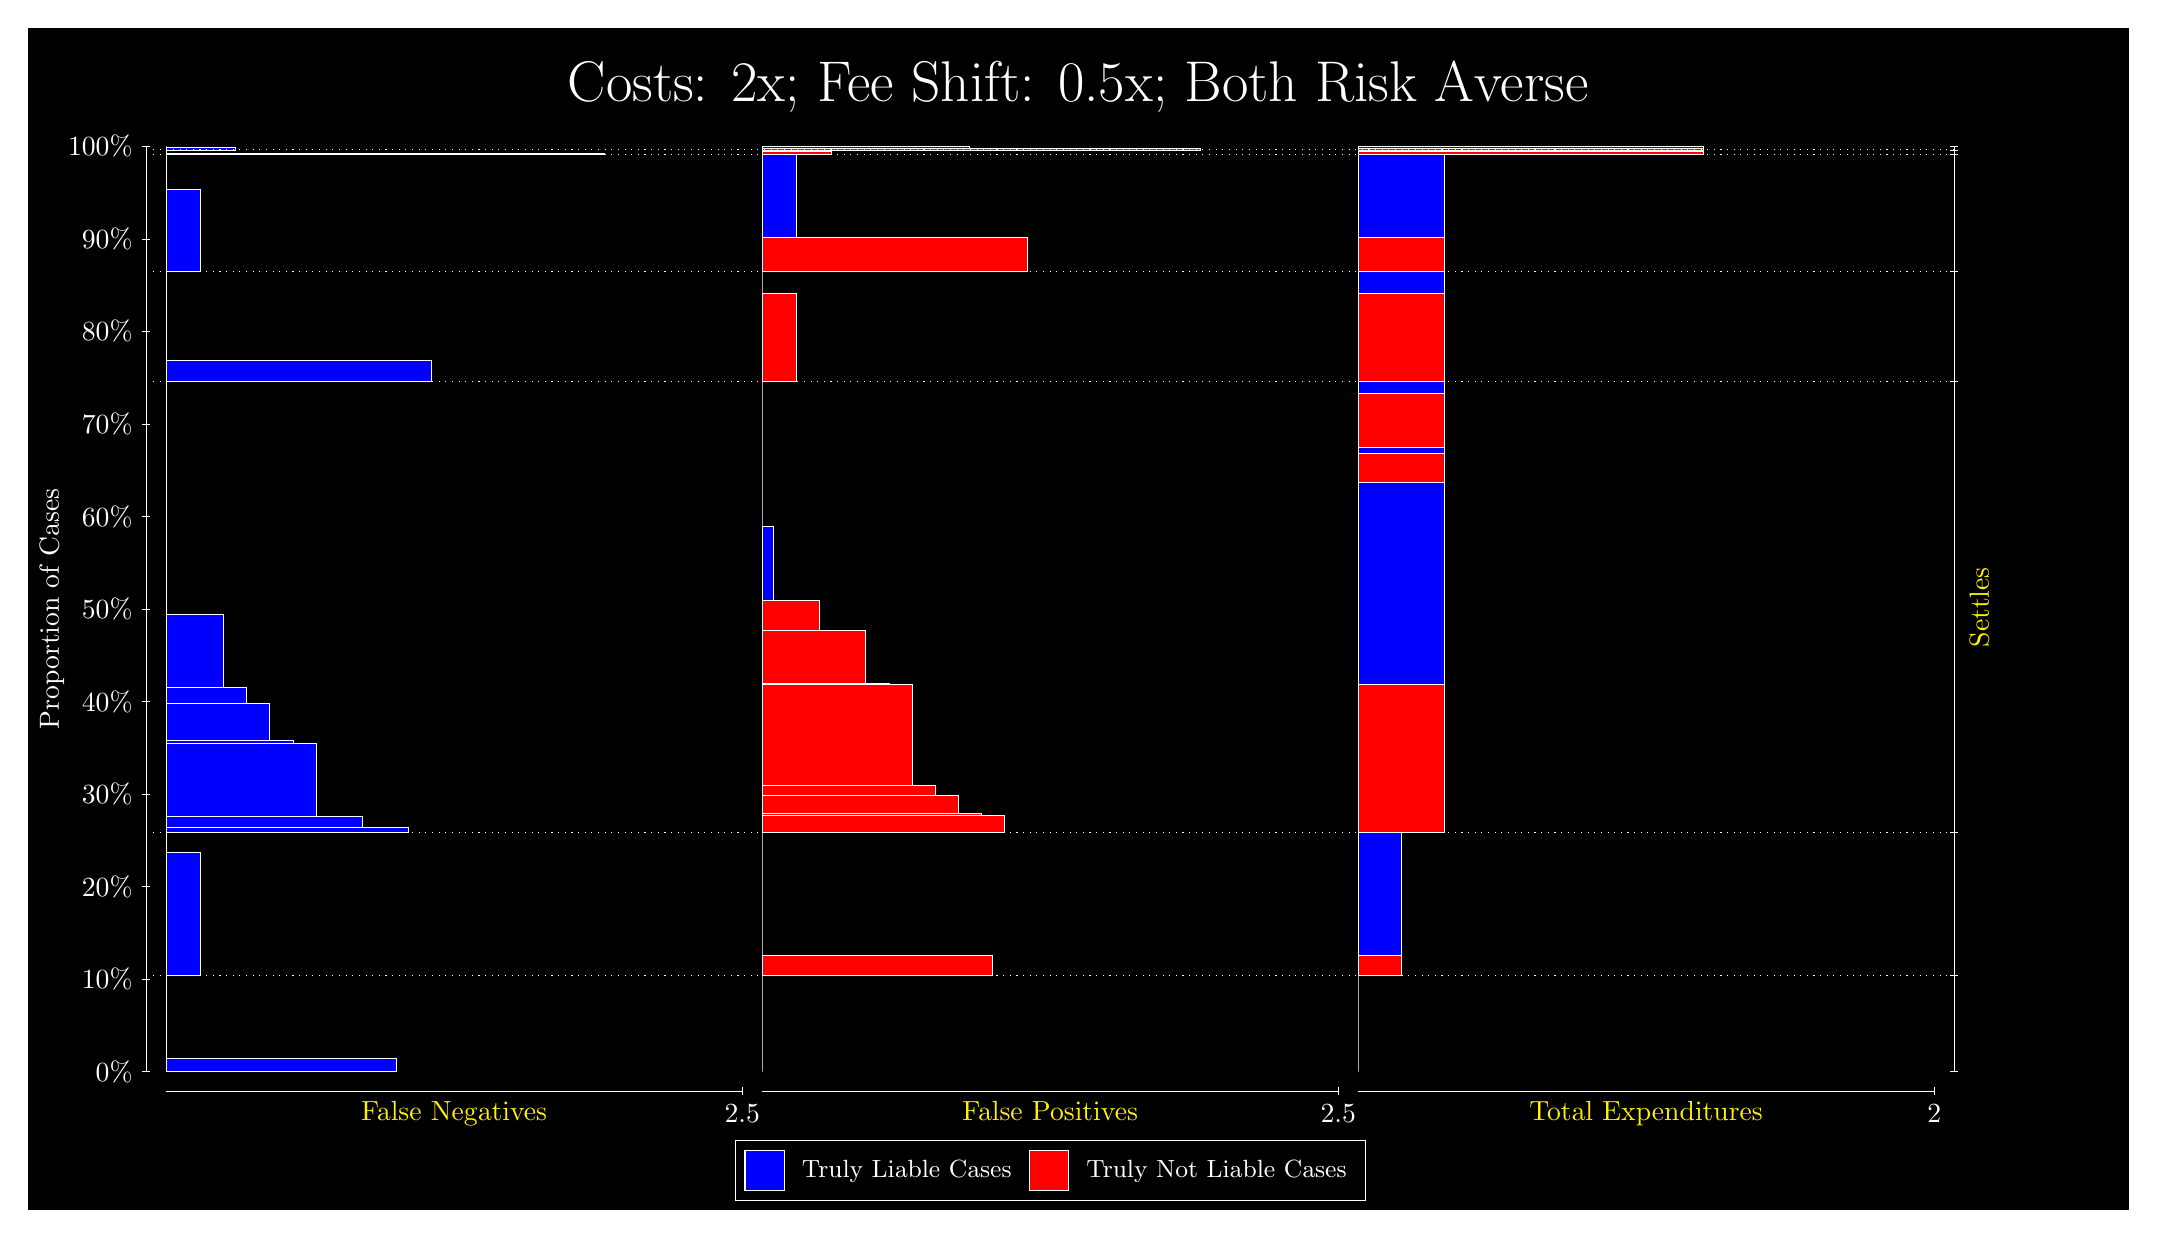
\begin{tikzpicture}
\draw[fill=black] (0,0) rectangle (26.667,15);
\draw[text=white] (0,13.5) rectangle (26.667,15) node[midway] {\huge Costs: 2x; Fee Shift: 0.5x; Both Risk Averse};
\draw[white, very thin] (1.5,1.75) -- (1.5,13.5);
\node[rotate=90, text=white, anchor=center] at (0.3, 7.625) {Proportion of Cases};
\draw[white, very thin] (1.45,1.75) -- (1.55,1.75);
\node[text=white, anchor=east] at (1.45, 1.75) {0\%};
\draw[white, very thin] (1.45,2.925) -- (1.55,2.925);
\node[text=white, anchor=east] at (1.45, 2.925) {10\%};
\draw[white, very thin] (1.45,4.1) -- (1.55,4.1);
\node[text=white, anchor=east] at (1.45, 4.1) {20\%};
\draw[white, very thin] (1.45,5.275) -- (1.55,5.275);
\node[text=white, anchor=east] at (1.45, 5.275) {30\%};
\draw[white, very thin] (1.45,6.45) -- (1.55,6.45);
\node[text=white, anchor=east] at (1.45, 6.45) {40\%};
\draw[white, very thin] (1.45,7.625) -- (1.55,7.625);
\node[text=white, anchor=east] at (1.45, 7.625) {50\%};
\draw[white, very thin] (1.45,8.8) -- (1.55,8.8);
\node[text=white, anchor=east] at (1.45, 8.8) {60\%};
\draw[white, very thin] (1.45,9.975) -- (1.55,9.975);
\node[text=white, anchor=east] at (1.45, 9.975) {70\%};
\draw[white, very thin] (1.45,11.15) -- (1.55,11.15);
\node[text=white, anchor=east] at (1.45, 11.15) {80\%};
\draw[white, very thin] (1.45,12.325) -- (1.55,12.325);
\node[text=white, anchor=east] at (1.45, 12.325) {90\%};
\draw[white, very thin] (1.45,13.5) -- (1.55,13.5);
\node[text=white, anchor=east] at (1.45, 13.5) {100\%};

\draw[white, very thin] (24.457,1.75) -- (24.457,13.5);
\draw[white, very thin] (24.407,1.75) -- (24.507,1.75);
\node[anchor=west] at (24.407, 1.75) {};
\draw[white, very thin] (24.407,2.9733) -- (24.507,2.9733);
\node[anchor=west] at (24.407, 2.9733) {};
\draw[white, very thin] (24.407,4.7841) -- (24.507,4.7841);
\node[anchor=west] at (24.407, 4.7841) {};
\draw[white, very thin] (24.407,10.51) -- (24.507,10.51);
\node[anchor=west] at (24.407, 10.51) {};
\draw[white, very thin] (24.407,11.911) -- (24.507,11.911);
\node[anchor=west] at (24.407, 11.911) {};
\draw[white, very thin] (24.407,13.393) -- (24.507,13.393);
\node[anchor=west] at (24.407, 13.393) {};
\draw[white, very thin] (24.407,13.454) -- (24.507,13.454);
\node[anchor=west] at (24.407, 13.454) {};
\draw[white, very thin] (24.407,13.5) -- (24.507,13.5);
\node[anchor=west] at (24.407, 13.5) {};

\draw[white, very thin, fill=blue] (1.75,1.75) rectangle (4.6775,1.9225);
\draw[white, very thin, fill=red] (1.75,1.9225) rectangle (1.75,2.9733);
\draw[white, very thin, fill=blue] (1.75,2.9733) rectangle (2.1891,4.5309);
\draw[white, very thin, fill=red] (1.75,4.5309) rectangle (1.75,4.7841);
\draw[white, very thin, fill=blue] (1.75,4.7841) rectangle (4.8239,4.8485);
\draw[white, very thin, fill=blue] (1.75,4.8485) rectangle (4.2384,4.9861);
\draw[white, very thin, fill=blue] (1.75,4.9861) rectangle (3.9457,4.9969);
\draw[white, very thin, fill=blue] (1.75,4.9969) rectangle (3.6529,5.9212);
\draw[white, very thin, fill=blue] (1.75,5.9212) rectangle (3.3602,5.9626);
\draw[white, very thin, fill=blue] (1.75,5.9626) rectangle (3.0674,6.429);
\draw[white, very thin, fill=blue] (1.75,6.429) rectangle (2.7746,6.6247);
\draw[white, very thin, fill=blue] (1.75,6.6247) rectangle (2.4819,7.5604);
\draw[white, very thin, fill=red] (1.75,7.5604) rectangle (1.75,10.51);
\draw[white, very thin, fill=blue] (1.75,10.51) rectangle (5.1167,10.788);
\draw[white, very thin, fill=red] (1.75,10.788) rectangle (1.75,11.911);
\draw[white, very thin, fill=blue] (1.75,11.911) rectangle (2.1891,12.956);
\draw[white, very thin, fill=red] (1.75,12.956) rectangle (1.75,13.393);
\draw[white, very thin, fill=blue] (1.75,13.393) rectangle (7.3123,13.41);
\draw[white, very thin, fill=red] (1.75,13.41) rectangle (1.75,13.454);
\draw[white, very thin, fill=blue] (1.75,13.454) rectangle (2.6283,13.484);
\draw[white, very thin, fill=red] (1.75,13.484) rectangle (1.75,13.5);
\draw[white, very thin, fill=red] (9.3189,1.75) rectangle (9.3189,2.8008);
\draw[white, very thin, fill=blue] (9.3189,2.8008) rectangle (9.3189,2.9733);
\draw[white, very thin, fill=red] (9.3189,2.9733) rectangle (12.246,3.2265);
\draw[white, very thin, fill=blue] (9.3189,3.2265) rectangle (9.3189,4.7841);
\draw[white, very thin, fill=red] (9.3189,4.7841) rectangle (12.393,5.0024);
\draw[white, very thin, fill=red] (9.3189,5.0024) rectangle (12.1,5.0291);
\draw[white, very thin, fill=red] (9.3189,5.0291) rectangle (11.807,5.2643);
\draw[white, very thin, fill=red] (9.3189,5.2643) rectangle (11.515,5.385);
\draw[white, very thin, fill=red] (9.3189,5.385) rectangle (11.222,6.6667);
\draw[white, very thin, fill=red] (9.3189,6.6667) rectangle (10.929,6.6813);
\draw[white, very thin, fill=red] (9.3189,6.6813) rectangle (10.636,7.356);
\draw[white, very thin, fill=red] (9.3189,7.356) rectangle (10.051,7.7337);
\draw[white, very thin, fill=blue] (9.3189,7.7337) rectangle (9.4652,8.6694);
\draw[white, very thin, fill=blue] (9.3189,8.6694) rectangle (9.3189,10.51);
\draw[white, very thin, fill=red] (9.3189,10.51) rectangle (9.758,11.633);
\draw[white, very thin, fill=blue] (9.3189,11.633) rectangle (9.3189,11.911);
\draw[white, very thin, fill=red] (9.3189,11.911) rectangle (12.686,12.349);
\draw[white, very thin, fill=blue] (9.3189,12.349) rectangle (9.758,13.393);
\draw[white, very thin, fill=red] (9.3189,13.393) rectangle (10.197,13.438);
\draw[white, very thin, fill=blue] (9.3189,13.438) rectangle (9.3189,13.454);
\draw[white, very thin, fill=red] (9.3189,13.454) rectangle (14.881,13.471);
\draw[white, very thin, fill=blue] (9.3189,13.471) rectangle (11.954,13.5);
\draw[white, very thin, fill=red] (16.888,1.75) rectangle (16.888,2.8008);
\draw[white, very thin, fill=blue] (16.888,2.8008) rectangle (16.888,2.9733);
\draw[white, very thin, fill=red] (16.888,2.9733) rectangle (17.437,3.2265);
\draw[white, very thin, fill=blue] (16.888,3.2265) rectangle (17.437,4.7841);
\draw[white, very thin, fill=red] (16.888,4.7841) rectangle (17.986,6.6667);
\draw[white, very thin, fill=blue] (16.888,6.6667) rectangle (17.986,9.2302);
\draw[white, very thin, fill=red] (16.888,9.2302) rectangle (17.986,9.6078);
\draw[white, very thin, fill=blue] (16.888,9.6078) rectangle (17.986,9.6722);
\draw[white, very thin, fill=red] (16.888,9.6722) rectangle (17.986,10.362);
\draw[white, very thin, fill=blue] (16.888,10.362) rectangle (17.986,10.51);
\draw[white, very thin, fill=red] (16.888,10.51) rectangle (17.986,11.633);
\draw[white, very thin, fill=blue] (16.888,11.633) rectangle (17.986,11.911);
\draw[white, very thin, fill=red] (16.888,11.911) rectangle (17.986,12.349);
\draw[white, very thin, fill=blue] (16.888,12.349) rectangle (17.986,13.393);
\draw[white, very thin, fill=red] (16.888,13.393) rectangle (21.279,13.438);
\draw[white, very thin, fill=blue] (16.888,13.438) rectangle (21.279,13.454);
\draw[white, very thin, fill=red] (16.888,13.454) rectangle (21.279,13.471);
\draw[white, very thin, fill=blue] (16.888,13.471) rectangle (21.279,13.5);
\draw[white, dotted] (1.5,2.9733) -- (24.457,2.9733);
\draw[white, dotted] (1.5,4.7841) -- (24.457,4.7841);
\draw[white, dotted] (1.5,10.51) -- (24.457,10.51);
\draw[white, dotted] (1.5,11.911) -- (24.457,11.911);
\draw[white, dotted] (1.5,13.393) -- (24.457,13.393);
\draw[white, dotted] (1.5,13.454) -- (24.457,13.454);
\draw[white, very thin] (1.75,1.5) -- (9.0689,1.5);
\node[text=yellow, anchor=north] at (5.4094, 1.5) {False Negatives};
\draw[white, very thin] (9.0689,1.45) -- (9.0689,1.55);
\node[text=white, anchor=north] at (9.0689, 1.45) {2.5};

\draw[white, very thin] (9.3189,1.5) -- (16.638,1.5);
\node[text=yellow, anchor=north] at (12.978, 1.5) {False Positives};
\draw[white, very thin] (16.638,1.45) -- (16.638,1.55);
\node[text=white, anchor=north] at (16.638, 1.45) {2.5};

\draw[white, very thin] (16.888,1.5) -- (24.207,1.5);
\node[text=yellow, anchor=north] at (20.547, 1.5) {Total Expenditures};
\draw[white, very thin] (24.207,1.45) -- (24.207,1.55);
\node[text=white, anchor=north] at (24.207, 1.45) {2};



\node[text=yellow, centered, rotate=90] at (24.777, 7.647) {Settles};





\draw (12.978300999999998,1.5) node[draw=none] (baseCoordinate) {};
\begin{scope}[align=center]
        \matrix[scale=0.5, draw=white, below=0.5cm of baseCoordinate, nodes={draw}, column sep=0.1cm]{
            \node[rectangle, draw, minimum width=0.5cm, minimum height=0.5cm, fill=blue] {}; &
            \node[draw=none, font=\small, text=white] (B) {Truly Liable Cases}; &
            \node[rectangle, draw, minimum width=0.5cm, minimum height=0.5cm, fill=red] {}; &
            \node[draw=none, font=\small, text=white] (B) {Truly Not Liable Cases}; \\
            };
\end{scope}

\end{tikzpicture}
\end{document}